%!TEX root = thesis.tex
\chapter{Methodik und Experimentelles Vorgehen}
\label{chapter-konzept}

In diesem Kapitel wird das methodische Vorgehen der vorliegenden
Arbeit beschrieben. Ziel der experimentellen Untersuchung ist es,
zu analysieren, inwieweit Large Language Models (LLMs) zur
Rekonstruktion eines bestehenden Softwaresystems eingesetzt werden
können.

Hierzu wird ein bestehendes Legacy-System analysiert und auf Basis
seiner Anforderungen mithilfe verschiedener LLM-Modelle neu
generiert. Die resultierenden Systeme werden anschließend
systematisch bewertet und miteinander verglichen.

\section{Untersuchungdesign}
Die Untersuchung folgt einem experimentellen Ansatz.
Als Fallstudie dient das Buchungssystem \textit{Passat}.
Zunächst wurden die funktionalen Anforderungen des
Legacy-Systems analysiert und strukturiert aufbereitet.

Auf Basis dieser Anforderungen wurden verschiedene
Prompt-Varianten entwickelt, die anschließend in mehrere
Large Language Models eingegeben wurden, um neue
Implementierungen des Systems zu generieren.

Insgesamt wurde das System neunmal generiert, wobei
unterschiedliche Kombinationen aus LLM-Modellen und
Prompt-Varianten verwendet wurden. Ziel ist es, die
Unterschiede zwischen den generierten Systemen zu
analysieren und zu bewerten, inwieweit die ursprünglichen
Anforderungen erfüllt werden.



\section{Ausgangssystem (Legacy-System Passat)}
Als Fallstudie für die experimentelle Untersuchung wurde das
Legacy-System \textit{Passat} verwendet. Passat ist ein webbasiertes
Buchungs- und Reservierungssystem, das zur Verwaltung
raumähnlicher Ressourcen in kleinen Hotels oder Pensionen
entwickelt wurde. Ziel des Systems ist es, die Verwaltung von
Reservierungen, Buchungen und Kundeninformationen zu
unterstützen.

Das System bietet eine Vielzahl von Funktionen, darunter die
Verwaltung von Buchungen und Reservierungen, die Speicherung
von Kundendaten sowie die Erstellung von Rechnungen. Darüber
hinaus verfügt das System über ein Kalendermodul zur Darstellung
der aktuellen Raumbelegung sowie über einen dynamischen
Preiskatalog zur Verwaltung zeitabhängiger Preise. Zusätzlich
unterstützt das System verschiedene Nutzerrollen und
Rechtestrukturen, wodurch unterschiedliche Benutzergruppen
verschiedene Funktionen des Systems nutzen können.

Technisch basiert das System auf einer klassischen
Client-Server-Architektur. Die Serverkomponente läuft auf einem
Application Server und verwendet eine relationale Datenbank
zur Speicherung der Systemdaten. Die Clientkomponente wird
über ein webbasiertes Benutzerinterface im Browser verwendet
und benötigt keine lokale Installation.

Aufgrund seiner klar definierten Anforderungen, seiner
umfangreichen Funktionalitäten sowie der vorhandenen
Dokumentation eignet sich das System Passat als geeignete
Fallstudie zur Untersuchung der automatischen
Systemgenerierung mithilfe von Large Language Models.

\subsection{Konzeptionelles Datenmodell des Buchungssystems}

Die folgende Abbildung zeigt das konzeptionelle
Datenmodell des Buchungssystems in Form eines
UML-Klassendiagramms. Das Modell beschreibt die
zentralen Entitäten sowie deren Beziehungen und
bildet die fachliche Struktur des Systems ab.

Zentrales Element ist die Entität \textit{Order}, die
einen vollständigen Buchungsvorgang repräsentiert.
Eine Order besteht aus mehreren \textit{OrderItems},
welche jeweils einzelne Buchungseinträge mit einem
definierten Zeitraum (von/bis) darstellen. Ein
OrderItem beschreibt somit die konkrete Nutzung
einer Ressource innerhalb eines bestimmten Zeitraums.

Die tatsächlich buchbaren Ressourcen werden durch die
abstrakte Entität \textit{Orderable} modelliert. Diese
dient als Oberklasse für unterschiedliche Ressourcentypen,
wie beispielsweise \textit{Room} oder \textit{Special}.
Durch diese Generalisierung wird eine flexible Erweiterung
des Systems ermöglicht, da neue buchbare Objekte ohne
grundlegende Änderungen integriert werden können.

Ergänzend unterstützt das Modell sogenannte
\textit{Additions}, welche optionale Zusatzleistungen
repräsentieren, die einem OrderItem zugeordnet werden
können. Beispiele hierfür sind zusätzliche Ausstattungen
oder Serviceleistungen. Die Verfügbarkeit dieser Additions
kann entweder begrenzt oder, im Falle entsprechender
Kennzeichnung (z.\,B. durch ein \textit{infinity\_flag}),
unbegrenzt sein.

Die Beziehungen zwischen den Entitäten folgen einem
hierarchischen Aufbau: Eine Order aggregiert mehrere
OrderItems, während jedes OrderItem genau einem
Orderable zugeordnet ist. Additions erweitern einzelne
OrderItems und ermöglichen eine detaillierte Modellierung
komplexer Buchungsszenarien.

Das dargestellte Modell folgt grundlegenden Prinzipien
der objektorientierten Modellierung, insbesondere der
Abstraktion, Generalisierung sowie der Aggregation und
Komposition, und stellt eine zentrale Grundlage für die
funktionale Struktur des Buchungssystems dar.



Wie in Abbildung \ref{fig:buchungssystem} dargestellt, zeigt das Diagramm die Struktur des Buchungssystems.
\begin{figure}[h]
    \centering
    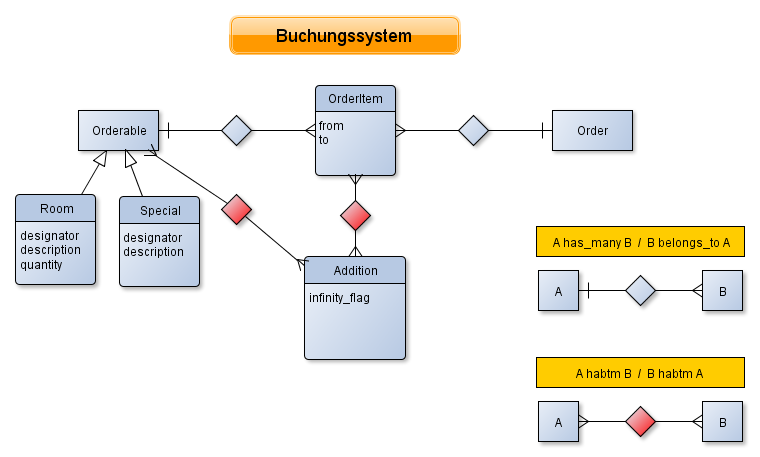
\includegraphics[width=0.8\textwidth]{images/buchungssystem.png}
  \caption{UML-Klassendiagramm des konzeptionellen Datenmodells des Buchungssystems (Darstellung in Anlehnung an Schmalz \cite{Schmalz2026}).}
    \label{fig:buchungssystem}
\end{figure}


\subsection{Analyse der Anforderungen und Spezifikation}
Die Analyse der Anforderungen basiert auf der vorhandenen
Dokumentation des Legacy-Systems \textit{Passat}, die sowohl
eine detaillierte Anforderungsbeschreibung als auch
funktionale Spezifikationen umfasst. Da das System nicht
öffentlich zugänglich ist, wurden zusätzliche Informationen
durch den ursprünglichen Entwickler des Systems erhoben.

Der Entwickler diente dabei als fachlicher Ansprechpartner,
um Unklarheiten in der bestehenden Dokumentation zu klären
und die ursprünglichen Systemanforderungen zu validieren.
Diese Kombination aus Dokumentenanalyse und Expertenwissen
ermöglicht eine konsistente und nachvollziehbare
Rekonstruktion der Anforderungen \cite{Schmalz2026}.

Im Rahmen der Analyse wurden die Anforderungen zunächst
extrahiert und anschließend in strukturierter Form
aufbereitet. Aufgrund der teilweise heterogenen und
umfangreichen Originalbeschreibung wurden die Anforderungen
konsolidiert, zusammengefasst und in mehrere Varianten
überführt. Ziel dieser Variantenbildung war es, unterschiedliche
Darstellungsformen der Spezifikation zu erzeugen, die als
Eingabe für die Large Language Models verwendet werden können.

Dabei wurden die ursprünglichen funktionalen Anforderungen
nicht verändert, sondern ausschließlich in strukturierter und
für die weitere Verarbeitung geeigneter Form dargestellt.

\section{Prompt Engineering und Prompt-Varianten}

Die Generierung der Softwaresysteme basiert auf dem
Einsatz von Prompt Engineering, welches die gezielte
Gestaltung von Eingaben für Large Language Models
beschreibt \cite{boonstra2024prompt}.

Die Prompts wurden auf Grundlage der analysierten
Systemanforderungen entwickelt. Dabei kamen insbesondere
Contextual Prompting sowie strukturierte
Promptformulierungen zum Einsatz. Ziel war es, dem Modell
ein möglichst vollständiges Verständnis der Systemdomäne
zu vermitteln.


\subsection{Prompting für Codegenerierung}


Die Generierung von Programmcode stellt eine zentrale
Anwendung von LLMs dar. Effektive Prompts bestehen dabei
aus einer klaren Aufgabenbeschreibung, einer strukturierten
Darstellung der Logik sowie einer expliziten Aufforderung
zur Generierung des Codes.

Darüber hinaus ist die Validierung des generierten Codes
von entscheidender Bedeutung. Hierzu wurde der erzeugte
Code gespeichert, ausgeführt und hinsichtlich seiner
Funktionalität überprüft.

\subsection{Definition der Prompt-Varianten}

Zur Untersuchung wurden drei Prompt-Varianten mit
unterschiedlichem Komplexitätsgrad definiert:

\begin{itemize}
\item \textbf{Prompt 1}: Einfacher Basis-Prompt ohne Struktur
\item \textbf{Prompt 2}: Strukturierter Prompt mit Kontextinformationen
\item \textbf{Prompt 3}: Erweiterter Prompt mit Role Prompting
\end{itemize}

Ziel ist es, den Einfluss der Promptstruktur auf die
Qualität der generierten Systeme zu analysieren.

\section{Eingesetzte LLM-Modelle}

In dieser Arbeit wurden folgende Modelle verwendet:

\begin{itemize}
\item GPT Codex 5.1 Max
\item Gemini 3.1 Pro
\item GPT 5.2
\end{itemize}

Die Auswahl der Modelle erfolgte mit dem Ziel, unterschiedliche Fähigkeiten moderner Large Language Models (LLMs) abzudecken. Alle eingesetzten Modelle basieren auf der Transformer-Architektur, unterscheiden sich jedoch hinsichtlich ihrer Spezialisierung und ihres Anwendungsschwerpunkts.

GPT Codex 5.1 Max ist ein auf Softwareentwicklung spezialisiertes Modell. Es wurde gezielt auf große Mengen von Quellcode sowie technische Dokumentationen trainiert und ist insbesondere für Aufgaben wie Codegenerierung, Codeanalyse und automatische Vervollständigung geeignet. Durch sein tiefes Verständnis formaler Sprachen ermöglicht es eine effiziente Unterstützung im Entwicklungsprozess sowie die Übersetzung von natürlichsprachlichen Anforderungen in ausführbaren Code.

Gemini 3.1 Pro ist ein multimodales Modell, das neben Text auch weitere Datentypen wie Bilder und strukturierte Informationen verarbeiten kann. Der Fokus liegt auf der Integration und Analyse unterschiedlicher Informationsquellen. Dadurch eignet sich das Modell besonders für komplexe Aufgabenstellungen, bei denen ein kontextübergreifendes Verständnis erforderlich ist.

GPT 5.2 stellt ein generalistisches Sprachmodell dar, das für eine breite Palette von Aufgaben der natürlichen Sprachverarbeitung eingesetzt wird. Dazu zählen unter anderem Textgenerierung, Zusammenfassung, semantische Analyse sowie logisches Schlussfolgern. Das Modell zeichnet sich durch eine hohe Kontextverarbeitungskapazität und robuste Generalisierungsfähigkeit aus.

Durch die Kombination dieser drei Modelle wird sowohl eine breite Abdeckung allgemeiner Sprachverarbeitungsaufgaben als auch eine Spezialisierung auf technische und multimodale Anwendungsfälle erreicht. Dies ermöglicht eine differenzierte Analyse und Nutzung der jeweiligen Modellstärken im Rahmen dieser Arbeit.

\section{Technische Umgebung}

Die generierten Systeme wurden mit der Programmiersprache
Python und dem Webframework Django umgesetzt. Ziel war es,
die Fähigkeit der LLMs zur Generierung vollständiger
Webanwendungen zu untersuchen.

Zur Entwicklung und Auswertung wurde eine integrierte
Entwicklungsumgebung verwendet, die eine direkte
Interaktion mit den LLMs sowie die Ausführung des Codes
ermöglichte.

\section{Versuchaufbau}

Der Versuchsaufbau basiert auf der Kombination von drei
Prompt-Varianten mit drei verschiedenen LLM-Modellen.

\begin{center}
Prompt 1–3 $\times$ 3 Modelle = 9 Experimente
\end{center}

Jede Kombination wurde verwendet, um ein vollständiges
System zu generieren und anschließend zu analysieren.

\section{Durchführung der Experiment}

Die Experimente wurden durchgeführt, indem die definierten
Prompts in die jeweiligen LLM-Systeme eingegeben wurden.
Die generierten Ergebnisse wurden anschließend gespeichert,
ausgeführt und systematisch überprüft.

Dabei wurden zentrale Anwendungsfälle getestet, wie die
Verwaltung von Kunden, Buchungen sowie die Interaktion
über die Benutzeroberfläche.

Die Ergebnisse wurden dokumentiert und für die
anschließende Auswertung vorbereitet.

\section{Evaluationskriterien}

Zur Bewertung der generierten Systeme wurden funktionale
und qualitative Kriterien definiert.

Zu den funktionalen Kriterien zählt insbesondere die
korrekte Umsetzung der Anforderungen. Ergänzend wurden
qualitative Aspekte wie Codequalität, Architektur sowie
die Benutzeroberfläche bewertet.

Die Bewertung erfolgt anhand eines Punktesystems, um eine
vergleichbare Analyse der generierten Systeme zu
ermöglichen.


\section{Effizienzsteigerung durch strukturierte Prompts bei LLMs}

Große Sprachmodelle (Large Language Models, LLMs)
werden zunehmend für komplexe Aufgaben wie
Softwareentwicklung oder Anforderungsanalyse eingesetzt.

Die Qualität der generierten Ergebnisse hängt dabei
stark von der Struktur der Eingabeaufforderung
(Prompt) ab.

Insbesondere bei umfangreichen Eingaben ist eine
Aufteilung in kleinere, klar definierte Aufgabenbereiche
deutlich effektiver als ein einzelner komplexer Prompt.

Ein zentrales Problem bei langen Eingaben ist die
ungleiche Gewichtung von Informationen innerhalb des
Modells.

Relevante Inhalte können dadurch in den Hintergrund
treten, während weniger wichtige Informationen stärker
berücksichtigt werden.

Dies führt häufig zu unvollständigen oder inkorrekten
Ergebnissen.

Darüber hinaus erhöht eine hohe Informationsdichte die
kognitive Komplexität der Aufgabe.

Wenn mehrere Aufgaben gleichzeitig verarbeitet werden
müssen, kann es zu Interferenzeffekten kommen.

Dabei konkurrieren verschiedene Teilaufgaben um die
begrenzten Ressourcen des Modells.

Die Aufteilung in mehrere Schritte (z.\,B. Analyse
$\rightarrow$ Validierung $\rightarrow$ Implementierung)
ermöglicht hingegen eine klare Fokussierung.

Dieses Vorgehen wird als ``Prompt Chaining'' oder
``Decomposition'' bezeichnet.

Studien zeigen, dass diese Strategien die Qualität und
Konsistenz der Ergebnisse verbessern können.

Ein weiterer Vorteil besteht darin, dass
Zwischenergebnisse sichtbar gemacht werden.

Dadurch können Fehler frühzeitig erkannt und korrigiert
werden.

Insgesamt verbessert die strukturierte Aufteilung die
Leistungsfähigkeit von Sprachmodellen deutlich.




\section{Evaluationskriterien}

Zur systematischen Bewertung der generierten Softwaresysteme
wurden in dieser Arbeit sowohl funktionale als auch
qualitative Evaluationskriterien definiert. Ziel ist es,
die durch verschiedene Large Language Models erzeugten
Systeme objektiv vergleichbar zu machen.

Die Auswahl der Kriterien basiert auf etablierten
Softwarequalitätsmodellen, insbesondere ISO/IEC 9126 sowie
dem FURPS-Modell, welche Softwarequalität als
multidimensionales Konzept beschreiben. Diese Modelle
bilden die Grundlage für eine strukturierte und
nachvollziehbare Bewertung.

In dieser Arbeit wurden die folgenden zentralen Kriterien
herangezogen:

\begin{itemize}
    \item \textbf{Funktionalität}: Bewertung der Umsetzung
    der definierten Anforderungen, insbesondere der
    Buchungsverwaltung, Kundenverwaltung sowie der
    Benutzerrollen.

    \item \textbf{Vollständigkeit}: Grad der Abdeckung der
    ursprünglichen Anforderungen des Legacy-Systems.

    \item \textbf{Codequalität}: Struktur, Lesbarkeit und
    Nachvollziehbarkeit des generierten Codes.

    \item \textbf{Architektur}: Einhaltung der
    Django-spezifischen Struktur (Model-View-Template),
    sowie die sinnvolle Aufteilung der Systemkomponenten.

    \item \textbf{Benutzeroberfläche (GUI)}:
    Benutzerfreundlichkeit, Struktur und Interaktion
    des generierten Webinterfaces.
\end{itemize}

Zur Vergleichbarkeit der Ergebnisse wurde ein
Punktesystem eingeführt, bei dem jedes Kriterium auf
einer Skala bewertet wird. Dies ermöglicht eine
quantitative Analyse der generierten Systeme und
eine objektive Gegenüberstellung der verschiedenen
LLM-Modelle und Prompt-Varianten.

\section{Einfluss strukturierter Prompts auf die Ergebnisqualität}

Die Qualität der durch Large Language Models generierten
Ergebnisse hängt maßgeblich von der Struktur der Eingabe
(Prompt) ab. Insbesondere bei komplexen Aufgaben wie der
automatischen Generierung von Softwaresystemen spielt die
Gestaltung der Prompts eine entscheidende Rolle.

Ein wesentliches Problem bei umfangreichen Prompts ist die
ungleiche Gewichtung von Informationen innerhalb des
Modells. Wichtige Anforderungen können dadurch weniger
stark berücksichtigt werden, während weniger relevante
Informationen stärker in die Generierung einfließen.

Darüber hinaus erhöht eine hohe Informationsdichte die
Komplexität der Aufgabe für das Modell. Werden mehrere
Aufgaben gleichzeitig gestellt, kann es zu
Interferenzeffekten kommen, bei denen verschiedene
Teilaufgaben miteinander konkurrieren.

Eine bewährte Strategie zur Verbesserung der Ergebnisse
besteht daher in der strukturierten Aufteilung komplexer
Prompts in mehrere Teilaufgaben. Dieser Ansatz wird in der
Literatur als \textit{Prompt Chaining} oder
\textit{Decomposition} bezeichnet.

Durch die schrittweise Bearbeitung einzelner Aufgaben
kann das Modell gezielter arbeiten, wodurch die Qualität
und Konsistenz der Ergebnisse verbessert wird. Zudem
ermöglicht dieser Ansatz die Analyse von
Zwischenergebnissen, wodurch Fehler frühzeitig erkannt
und korrigiert werden können.


\section{Versuchsaufbau}

Der Versuchsaufbau basiert auf der systematischen
Kombination von drei Promptvarianten mit
drei unterschiedlichen LLM-Modellen.

Es wurden drei Prompt-Varianten mit steigendem
Komplexitätsgrad definiert:

\begin{itemize}
    \item \textbf{Prompt 1}: Einfacher, unstrukturierter Prompt
    \item \textbf{Prompt 2}: Strukturierter Prompt mit Kontextinformationen
    \item \textbf{Prompt 3}: Erweiterter Prompt mit Role Prompting
\end{itemize}

Diese Prompts wurden jeweils in drei verschiedene
LLM-Modelle eingegeben:

\begin{itemize}
    \item GPT-5.2
    \item GPT Codex 5.1 Max
    \item Gemini 3.1 Pro
\end{itemize}

Insgesamt ergeben sich daraus neun Experimente, die eine
systematische Analyse des Einflusses von Promptstruktur
und Modellwahl ermöglichen.

\section{Durchführung der Experimente}

Die Durchführung der Experimente erfolgte in mehreren
Schritten. Zunächst wurden die definierten Prompts in die
jeweiligen LLM-Systeme eingegeben, um ein vollständiges
Softwaresystem zu generieren.

Der generierte Code wurde anschließend lokal gespeichert
und in einer geeigneten Entwicklungsumgebung ausgeführt.
Dabei wurden insbesondere Python und das Webframework
Django verwendet.

Im nächsten Schritt erfolgte die funktionale Überprüfung
der generierten Systeme. Hierbei wurden zentrale
Anwendungsfälle getestet, wie die Erstellung von Kunden,
die Verwaltung von Buchungen sowie die Interaktion über
die Benutzeroberfläche.

Abschließend wurden die Ergebnisse dokumentiert und auf
Basis der definierten Evaluationskriterien bewertet, um
eine vergleichende Analyse der verschiedenen Modelle und
Prompt-Varianten zu ermöglichen.
\section{Evaluation der mit Gemini 3.1 Pro generierten Systeme}
\subsection{Einfacher, unstrukturierter Prompt}

Im Folgenden wird das erste entwickelte System anhand der definierten Evaluationskriterien bewertet. Die Analyse basiert sowohl auf der Projektdokumentation als auch auf einer automatisierten Codeanalyse durch ein Large Language Model (LLM), welches den Quellcode (insbesondere \texttt{models.py}, \texttt{admin.py} und \texttt{views.py}) untersucht hat.

Das Projekt stellt ein Buchungs- und Reservierungssystem für kleine Unterkünfte dar. Die zentrale Domäne umfasst die Verwaltung von Zimmerkategorien, Zimmern, Kunden, Buchungen sowie Rechnungen. Die Implementierung basiert auf dem Django-Framework und nutzt insbesondere das integrierte Administrationsinterface als primäre Benutzerschnittstelle.

\subsection{Funktionalität}

Die grundlegenden funktionalen Anforderungen werden weitgehend erfüllt. Die Buchungsverwaltung ist durch ein entsprechendes Datenmodell mit Statusverfolgung (z.B. reserviert, bestätigt, eingecheckt) realisiert. Zudem besteht eine Verknüpfung zwischen Buchungen, Kunden und Zimmern. Eine einfache automatische Preisberechnung ist implementiert. Auch die Kundenverwaltung ist durch ein strukturiertes Datenmodell abgebildet.

Einschränkungen bestehen jedoch bei der Umsetzung der Benutzerrollen. Zwar wird das Standard-Berechtigungssystem von Django verwendet, jedoch fehlen spezifische, domänenspezifische Rollen mit differenzierter Logik.

\subsection{Vollständigkeit}

Das System deckt die wesentlichen Anforderungen eines klassischen Reservierungssystems ab. Die zentralen Entitäten und deren Beziehungen sind vollständig modelliert. Dennoch fehlen weiterführende Funktionen wie die Vermeidung von Doppelbuchungen durch komplexe Validierungslogik, eine vollständige Rechnungsverarbeitung (z.B. PDF-Generierung) sowie die Integration von Zahlungsprozessen. Somit ist die funktionale Abdeckung als weitgehend, jedoch nicht vollständig zu bewerten.

\subsection{Codequalität}

Die Codequalität ist insgesamt als hoch einzuschätzen. Die Datenmodelle sind klar strukturiert und folgen etablierten Best Practices des Django-Frameworks. Dazu gehören unter anderem die Verwendung von Auswahlfeldern (Choices), sprechenden Methoden zur String-Repräsentation sowie hilfreichen Metadaten. Auch die Konfiguration des Admin-Interfaces ist übersichtlich und unterstützt effiziente Datenverwaltung durch Filter- und Suchfunktionen.

\subsection{Architektur}

In Bezug auf die Softwarearchitektur zeigt sich eine gemischte Bewertung. Während die Datenmodellierung sauber umgesetzt ist, entspricht die Anwendung nicht vollständig dem Model-View-Template (MVT)-Paradigma von Django. Insbesondere fehlen eigene Views sowie Templates, wodurch keine klare Trennung zwischen Datenhaltung, Logik und Präsentation besteht. Das System basiert primär auf der Nutzung des Django-Admin-Interfaces und kann daher als prototypische Backend-Lösung eingeordnet werden.

\subsection{Benutzeroberfläche (GUI)}

Die Benutzeroberfläche basiert ausschließlich auf dem generischen Django-Admin-Interface. Dieses bietet zwar grundlegende Funktionalitäten wie Filter- und Suchoptionen, ist jedoch primär für technische Anwender konzipiert. Eine benutzerfreundliche, auf Endnutzer zugeschnittene Oberfläche mit spezifischen Interaktionskonzepten (z.B. Kalenderansichten oder Dashboards) ist nicht vorhanden. Daher ist die Usability für nicht-technische Nutzer eingeschränkt.

\subsection{Zusammenfassung}

Zusammenfassend handelt es sich bei dem Projekt um einen funktional soliden Backend-Prototyp mit einer qualitativ hochwertigen Datenmodellierung. Die größten Defizite liegen in der fehlenden Umsetzung einer eigenständigen Benutzeroberfläche sowie in der unvollständigen architektonischen Trennung der Anwendungsschichten. Für den produktiven Einsatz wären insbesondere Erweiterungen im Bereich der Benutzerinteraktion sowie der Geschäftslogik erforderlich.

\begin{table}[h]
\centering
\caption{Bewertung des ersten Projekts anhand definierter Kriterien}
\begin{tabular}{l c}
\hline
\textbf{Kriterium} & \textbf{Bewertung (0--5)} \\
\hline
Funktionalität & 4 \\
Vollständigkeit & 3 \\
Codequalität & 4 \\
Architektur & 3 \\
Benutzeroberfläche (GUI) & 2 \\
\hline
\textbf{Gesamt} & \textbf{16 / 25} \\
\hline
\end{tabular}
\end{table}

\subsection{Strukturierter Prompt mit Kontextinformationen}

Im Folgenden wird das zweite entwickelte System anhand der definierten Evaluationskriterien analysiert. Im Gegensatz zum ersten Projekt basiert diese Bewertung auf einer vollständigen Einsicht in die relevanten Quellcodedateien (insbesondere \texttt{models.py}, \texttt{views.py} sowie Templates), wodurch eine deutlich fundiertere Analyse möglich ist.

Das System stellt ein umfassendes Buchungs- und Verwaltungssystem dar, welches auf dem Django-Framework basiert und eine modulare Architektur mit mehreren Applikationen (u.a. \texttt{accounts}, \texttt{bookings}, \texttt{rooms}, \texttt{billing}, \texttt{tasks}) verwendet.

\subsection{Funktionalität}

Die funktionalen Anforderungen werden weitgehend erfüllt. Die Buchungsverwaltung ist durch ein flexibles Datenmodell mit Statusverwaltung (z.B. \textit{PENDING}, \textit{CONFIRMED}, \textit{CHECKED\_IN}, \textit{CHECKED\_OUT}) umgesetzt und bildet typische Abläufe eines Hotelbetriebs realistisch ab. Die Kundenverwaltung ist strukturiert implementiert und vermeidet durch geeignete Mechanismen (z.B. \texttt{get\_or\_create}) redundante Datensätze.

Besonders hervorzuheben ist die Erweiterung des Standard-Benutzermodells, wodurch spezifische Rollen wie Administrator, Rezeption und Reinigungspersonal abgebildet werden können. Einschränkungen bestehen jedoch in der fehlenden konsequenten Durchsetzung rollenbasierter Zugriffskontrollen in den Views.

\subsection{Vollständigkeit}

Das System weist eine hohe funktionale Abdeckung auf. Neben den Kernfunktionen eines Reservierungssystems (Buchungen, Kunden, Zimmer) werden zusätzliche Aspekte wie Abrechnung und Aufgabenverwaltung integriert. Die modulare Struktur erlaubt eine flexible Erweiterung und bildet komplexere Geschäftsprozesse eines Legacy-Systems umfassend ab.

\subsection{Codequalität}

Die Codequalität ist als sehr hoch zu bewerten. Der Quellcode ist übersichtlich strukturiert, folgt etablierten Django-Best-Practices und ist gut lesbar. Die Verwendung klar definierter Statuswerte, konsistenter Namenskonventionen sowie moderner Django-Funktionalitäten spricht für eine professionelle Implementierung.

Kleinere Schwächen bestehen lediglich in einzelnen Inkonsistenzen, wie etwa geringfügigen Formatierungsproblemen, die jedoch keinen signifikanten Einfluss auf die Wartbarkeit haben.

\subsection{Architektur}

Die Architektur stellt eine der größten Stärken des Projekts dar. Das Model-View-Template-Paradigma wird konsequent eingehalten. Die klare Trennung von Datenmodell, Geschäftslogik und Präsentationsschicht sorgt für eine hohe Wartbarkeit und Erweiterbarkeit.

Besonders positiv ist die Aufteilung in mehrere spezialisierte Django-Apps, wodurch eine lose Kopplung und hohe Modularität erreicht wird. Dieses Vorgehen entspricht den Best Practices moderner Django-Anwendungen.

\subsection{Benutzeroberfläche (GUI)}

Die Benutzeroberfläche ist modern und benutzerfreundlich gestaltet. Durch die Integration von Bootstrap wird ein responsives Layout gewährleistet. Zusätzlich ermöglicht die Verwendung von FullCalendar.js eine interaktive Darstellung von Buchungen in Kalenderform, was den praktischen Anforderungen im Anwendungsbereich entspricht.

Die Benutzerinteraktion ist durchdacht und unterstützt typische Arbeitsabläufe effizient. Insgesamt hebt sich die GUI deutlich von der rein administrativen Oberfläche des ersten Projekts ab.

\subsection{Zusammenfassung}

Zusammenfassend stellt das zweite Projekt eine deutlich weiterentwickelte und vollständigere Implementierung eines Buchungssystems dar als das erste Projekt. Insbesondere die saubere Architektur, die hohe Codequalität sowie die benutzerfreundliche Oberfläche machen das System zu einer nahezu produktionsreifen Anwendung.

Verbesserungspotenzial besteht vor allem in der konsequenten Umsetzung rollenbasierter Zugriffskontrollen sowie in kleineren Codeoptimierungen.


\begin{table}[h]
\centering
\caption{Bewertung des zweiten Projekts}
\begin{tabular}{l c}
\hline
\textbf{Kriterium} & \textbf{Bewertung (0--5)} \\
\hline
Funktionalität & 4 \\
Vollständigkeit & 4 \\
Codequalität & 4.5 \\
Architektur & 5 \\
Benutzeroberfläche (GUI) & 4.5 \\
\hline
\textbf{Gesamt} & \textbf{22 / 25} \\
\hline
\end{tabular}
\end{table}

\subsection{Erweiterter Prompt mit Role Prompting}

Im Folgenden wird das dritte entwickelte System anhand der definierten Evaluationskriterien analysiert. Die Bewertung basiert auf einer detaillierten Untersuchung des vollständigen Quellcodes, einschließlich der zentralen Komponenten \texttt{models.py}, \texttt{views.py}, sowie der implementierten Benutzeroberfläche.

Das Projekt stellt ein umfassendes Buchungs- und Verwaltungssystem dar, das auf dem Django-Framework basiert und sowohl administrative als auch operative Prozesse eines Hotelbetriebs digital abbildet.

\subsection{Funktionalität}

Die funktionalen Anforderungen werden in sehr hohem Maße erfüllt. Die Buchungsverwaltung bildet den gesamten Lebenszyklus einer Buchung ab, einschließlich verschiedener Statuszustände wie Option, Reservierung, Belegung und Stornierung. Besonders hervorzuheben ist die integrierte dynamische Preisberechnung, welche Aufenthaltsdauer sowie saisonale Preisanpassungen berücksichtigt.

Die Kundenverwaltung ist vollständig umgesetzt und enthält neben grundlegenden Informationen auch erweiterte Funktionen wie eine Blacklist-Logik. Das System nutzt zudem das integrierte Authentifizierungs- und Berechtigungssystem von Django, wodurch der Zugriff auf zentrale Funktionen eingeschränkt wird.

Darüber hinaus wurden zusätzliche Funktionen implementiert, die über die Grundanforderungen hinausgehen. Hierzu zählen ein Aufgabenverwaltungssystem für Mitarbeiter, eine Protokollierung von Systemaktivitäten (Audit-Logs) sowie die Möglichkeit zur Generierung von PDF-Rechnungen.

\subsection{Vollständigkeit}

Das System weist eine sehr hohe Abdeckung der Anforderungen eines klassischen Legacy-Buchungssystems auf. Neben den Kernfunktionen wie Zimmerverwaltung, Kundenmanagement und Buchungsprozessen werden auch Zusatzleistungen, saisonale Preisgestaltung sowie administrative und organisatorische Prozesse integriert.

Durch die Kombination dieser Funktionen wird ein umfassendes digitales Abbild eines klassischen Hotelverwaltungssystems erreicht, wodurch die Vollständigkeit als sehr hoch einzustufen ist.

\subsection{Codequalität}

Die Codequalität ist insgesamt als sehr hoch zu bewerten. Der Quellcode ist klar strukturiert, gut lesbar und folgt den etablierten Best Practices der Python- und Django-Entwicklung. Die Verwendung sprechender Bezeichner, klarer Modellstrukturen sowie gekapselter Logik (z.B. Preisberechnung innerhalb der Modelle) trägt maßgeblich zur Nachvollziehbarkeit bei.

Kleinere Schwächen bestehen lediglich in vereinzelten stilistischen Inkonsistenzen, die jedoch keinen signifikanten Einfluss auf die Wartbarkeit haben.

\subsection{Architektur}

Die Architektur des Systems ist durch eine klare Trennung der Verantwortlichkeiten gekennzeichnet und entspricht dem Model-View-Template-Paradigma des Django-Frameworks. Datenmodellierung, Geschäftslogik und Präsentationsschicht sind sauber voneinander getrennt.

Die Entscheidung, den Django-Admin-Bereich gezielt für administrative Aufgaben zu nutzen und gleichzeitig eigene Views und Templates für operative Prozesse bereitzustellen, stellt eine effiziente und praxisnahe Architektur dar.

\subsection{Benutzeroberfläche (GUI)}

Die Benutzeroberfläche ist funktional und auf die Anforderungen interner Anwender zugeschnitten. Dashboards, Tabellenansichten sowie interaktive Elemente ermöglichen eine effiziente Bedienung im Arbeitsalltag. Die Integration von Visualisierungskomponenten wie Diagrammen unterstützt zusätzlich die Analyse von Systemdaten.

Einschränkungen bestehen in der visuellen Gestaltung, da kein modernes CSS-Framework verwendet wird. Dadurch wirkt die Oberfläche im Vergleich zu aktuellen Webstandards weniger ansprechend, bleibt jedoch funktional und übersichtlich.

\subsection{Zusammenfassung}

Zusammenfassend stellt das dritte Projekt die ausgereifteste Implementierung im Vergleich der untersuchten Systeme dar. Es kombiniert eine hohe funktionale Abdeckung mit einer sauberen Architektur und guter Codequalität. Besonders hervorzuheben ist die Integration zusätzlicher Funktionen wie Audit-Logs, Aufgabenmanagement und dynamischer Preisberechnung.

Das System ist als nahezu produktionsreif einzuordnen, wobei Verbesserungen insbesondere im Bereich der Benutzeroberfläche möglich sind.

\begin{table}[h]
\centering
\caption{Bewertung des dritten Projekts}
\begin{tabular}{l c}
\hline
\textbf{Kriterium} & \textbf{Bewertung (0--5)} \\
\hline
Funktionalität & 5 \\
Vollständigkeit & 5 \\
Codequalität & 4.5 \\
Architektur & 4.5 \\
Benutzeroberfläche (GUI) & 4 \\
\hline
\textbf{Gesamt} & \textbf{23 / 25} \\
\hline
\end{tabular}
\end{table}

\subsection{Vergleich und Gesamtbewertung der entwickelten Systeme}

Im Rahmen dieser Arbeit wurden drei unterschiedliche Softwaresysteme unter Einsatz des Large Language Models Gemini 3.1 Pro generiert und analysiert. Ziel war es, die Fähigkeit des Modells zur Entwicklung komplexer Webanwendungen auf Basis des Django-Frameworks zu untersuchen. Die Bewertung erfolgte anhand der Kriterien Funktionalität, Vollständigkeit, Codequalität, Architektur sowie Benutzeroberfläche.

\subsection{Gemeinsamkeiten der Projekte}

Alle drei Systeme basieren auf dem Django-Framework und verfolgen das Ziel, ein Buchungs- und Verwaltungssystem für kleine Unterkünfte zu realisieren. In allen Fällen lassen sich zentrale Domänenobjekte identifizieren, darunter Zimmer, Kunden und Buchungen. Ebenso wurde durchgehend das integrierte Authentifizierungs- und Berechtigungssystem von Django verwendet.

Darüber hinaus zeigen alle Projekte, dass das LLM grundsätzlich in der Lage ist, konsistente Datenmodelle zu erzeugen und typische Geschäftsprozesse eines Reservierungssystems abzubilden. Insbesondere die Modellierung von Buchungszuständen sowie die Verknüpfung relevanter Entitäten sind in allen Projekten vorhanden.

\subsection{Unterschiede in Reifegrad und Umsetzung}

Trotz der konzeptionellen Gemeinsamkeiten unterscheiden sich die drei Projekte erheblich hinsichtlich ihres Reifegrads und ihrer technischen Umsetzung.

Das erste Projekt stellt primär einen Backend-Prototyp dar, der sich stark auf die Nutzung des Django-Admin-Interfaces konzentriert. Während die grundlegenden Datenstrukturen und Geschäftslogiken vorhanden sind, fehlt eine eigenständige Benutzeroberfläche sowie eine vollständige Umsetzung des Model-View-Template-Paradigmas. Das System ist daher als funktionaler, jedoch eingeschränkter Prototyp einzuordnen.

Das zweite Projekt zeigt eine deutlich fortgeschrittene Implementierung. Hier wurde das MVT-Paradigma konsequent umgesetzt, indem eigene Views, Templates sowie eine modulare Aufteilung in mehrere Django-Apps realisiert wurden. Zusätzlich wurde eine interaktive Benutzeroberfläche entwickelt, die durch moderne Webtechnologien wie Bootstrap und JavaScript-basierte Kalenderkomponenten erweitert wird. Dieses System kann als vollwertige Webanwendung betrachtet werden.

Das dritte Projekt stellt die ausgereifteste Lösung dar. Neben einer vollständigen Umsetzung der funktionalen Anforderungen wurden zusätzliche Features integriert, die über die Grundanforderungen hinausgehen. Dazu zählen unter anderem dynamische Preisberechnungen, Aufgabenmanagement, Aktivitätsprotokollierung sowie die Generierung von PDF-Rechnungen. Die Architektur ist klar strukturiert und entspricht modernen Best Practices. Auch wenn die Benutzeroberfläche funktional ist, weist sie im Vergleich zu aktuellen Webstandards leichte gestalterische Defizite auf.

\subsection{Vergleichende Analyse}

Die Entwicklung der drei Projekte zeigt eine deutliche Progression in der Qualität und Komplexität der generierten Systeme. Während das erste Projekt noch stark auf Standardfunktionalitäten des Frameworks angewiesen ist, demonstrieren die nachfolgenden Systeme eine zunehmende Fähigkeit des LLM, eigenständige und strukturierte Softwarelösungen zu erzeugen.

Besonders auffällig ist die Verbesserung in der Architektur und Modularität. Während im ersten Projekt keine klare Trennung der Anwendungsschichten erkennbar ist, wird diese im zweiten und dritten Projekt konsequent umgesetzt. Ebenso steigt die funktionale Tiefe der Systeme, insbesondere durch die Integration zusätzlicher Geschäftslogik und unterstützender Funktionen im dritten Projekt.

Die Benutzeroberfläche entwickelt sich ebenfalls weiter, von einer rein administrativen Oberfläche im ersten Projekt hin zu interaktiven und benutzerorientierten Interfaces in den nachfolgenden Systemen.

\subsection{Fazit}

Zusammenfassend lässt sich feststellen, dass das eingesetzte Large Language Model grundsätzlich in der Lage ist, komplexe Webanwendungen im Django-Kontext zu generieren. Die Qualität der Ergebnisse variiert jedoch deutlich und hängt stark von der jeweiligen Generierung sowie der bereitgestellten Kontextinformationen ab.

Während einfache Prototypen zuverlässig erzeugt werden können, erfordert die Entwicklung produktionsreifer Systeme eine präzisere Steuerung und Iteration. Die Ergebnisse zeigen jedoch, dass mit zunehmender Komplexität auch die Fähigkeit des Modells zur strukturierten und qualitativ hochwertigen Softwareentwicklung zunimmt.


\section{Quellen}

Quellen sind wichtig für gutes wissenschaftliches Arbeiten. Eine Quelle kann dabei zum Beispiel
\begin{compactitem}
  \item ein Beitrag in einer Zeitschrift \cite{MopOverview},
  \item ein Beitrag in einem Sammlungsband \cite{moore},
  \item ein Buch \cite{scala},
  \item ein Beitrag im Berichtsband einer Konferenz \cite{rltl},
  \item ein technischer Bericht \cite{bitkom},
  \item eine Dissertation \cite{Leucker02},
  \item eine Abschlussarbeit \cite{RltlConv},
  \item ein (noch) nicht veröffentlichter Artikel \cite{ptLTL} oder
  \item ein Artikel auf einer Website \cite{codecommit} sein.
  \item ein Survey-Artikel in einer Zeitschrift \cite{LLM4SE} sein.
  \item ein Artikel in einer Zeitschrift survey and openproblems \cite{LLM4SE2} sein.
  \item ein Buch \cite{sommerville2016software} sein.
  \item ein Buch \cite{seacord2003modernizing} sein.
  \item ein Artikel \cite{chikofsky1990reverse} sein.
  \item ein Artikel \cite{fan2023largelanguagemodelssoftware} sein.
  \item ein Artikel \cite{LLMinSEreviewandvision} sein.
  \item ein Artikel \cite{chen2021evaluatinglargelanguagemodels} sein.
  \item ein Artikel \cite{reynolds2021promptprogramminglargelanguage} sein.
  \item ein Artikel \cite{seemann2023ki} sein.
  \item ein Artikel auf einer Website \cite{zhang2023survey} sein.
  \item ein Buch \cite{boonstra2024prompt} sein.
  \item ein Artikel \cite{agarwal2024legacy} sein.
  \item eine Vorlesung \cite{leucker2024anforderungen} sein.
  \item eine Artikel \cite{brown2020languagemodelsfewshotlearners} sein.
  \item eine Artikel \cite{inproceedings} sein.  
  \item ein Artikel \cite{hou2024largelanguagemodelssoftware} sein.
  \item ein Personeninterview \cite{Schmalz2026} sein.
  \item ein Artikel auf einer whitepaper \cite{boonstra2023prompt} sein.
  \item ein Artikel auf einer whitepaper \cite{ray2024vibecoding} sein.
\end{compactitem}

Dabei ist zu beachten, dass nicht veröffentlichte Artikel und insbesondere Webseiten nur in Ausnahmefällen gute Quellen sind, da diese nicht durch Fachleute begutachtet wurden.

Im Bereich der Informatik können Quellenangaben im Bib\TeX-Format direkt der dblp\footnote{zum Beispiel \url{http://dblp.uni-trier.de}} entnommen werden.

\section{Tabellen}

In \vref{tbl-prozessoren} sehen wir ein Beispiel für eine Tabelle.

\begin{table}
  \centering
  \begin{zebratabular}{llr}
    \headerrow Jahr & Prozessor & MHz \\
    1975 & 6502 (C64) & 1 \\
    1985 & 80386 & 16 \\
    2005 & Pentium 4 & 2\,800 \\
    2030 & Phoenix 3 & 7\,320\,000 \\
    \hiderowcolors
    2050 & \ldots \\
    2070 & \ldots
  \end{zebratabular}
  \caption[Rechengeschwindigkeit von Computern]{Rechengeschwindigkeit von Computern. Inhaltlich vollkommen egal, ist dies doch ein sehr schönes Beispiel für eine Tabelle.}
  \label{tbl-prozessoren}
\end{table}

\section{Abbildungen und Diagramme}

In \vref{fig-flower} sehen wir ein Beispiel für eine Abbildung, die aus einer externen Grafik geladen wurde. In \vref{fig-buechi} sehen wir ein Beispiel für eine Abbildung, die in \LaTeX\ generiert wurde.

\begin{figure}
  \centering
  \pgfimage[width=.5\textwidth]{flower}
  \caption[Kurzfassung der Beschreibung für das Abbildungsverzeichnis]{Lange Version der Beschreibung, die direkt unter der Abbildung gesetzt wird. Es ist wichtig, für jede Abbildung eine umfangreiche Beschreibung anzugeben, da der Leser beim ersten Durchblättern der Arbeit vor allem an den Abbildungen hängen bleibt.}
  \label{fig-flower}
\end{figure}

\begin{figure}
  \centering
  \begin{tikzpicture}[
      node distance=15ex,
      auto,
      on grid,
      shorten >=1pt
    ]
    \node [state, initial] (q0) {$q_0$};
    \node [state, accepting, right=of q0] (q1) {$q_1$};
    \path[->]
      (q0) edge node {$a$} (q1);
  \end{tikzpicture}
  \caption[Graph des Büchi-Automaten $\hat A$.]{Graph des Büchi-Automaten $\hat A$. Der Zustand $q_1$ hat dabei keine ausgehende Kante. Der Zustand ist trotzdem akzeptierend, da beide enthaltenen Zustände von $\acute A$ akzeptierend sind. Die naive Anwendung des Leerheitstests auf alternierenden Büchi-Automaten liefert in diesem Fall also zu viele akzeptierende Zustände.}
  \label{fig-buechi}
\end{figure}

\section{Quelltext}

Quelltext sollte in Abschlussarbeiten nur äußerst sparsam eingesetzt werden. Wichtig ist insbesondere, dass Quelltextauszüge sorgsam ausgewählt und gut erklärt werden.

\begin{lstlisting}[language=Java,gobble=2]
  public class Main {
    // Hello Word in Java
    public static void main(String[] args) {
      System.out.println("Hello World");
    }
  }
\end{lstlisting}

\subsection{Quelltext mit automatischer Nummerierung}

Manchmal möchte man Quelltext eher als Abbildung und nicht als Fließtext behandeln. In diesem Fall soll der Quelltext eine Bildunterschrift und eine automatische Nummerierung erhalten. Die automatische Nummerierung kann dann natürlich auch in Referenzen verwendet werden: In \vref{lst:java} haben wir Java-Quelltext.

\begin{lstlisting}[language=Java,gobble=2,caption={Ich bin die Bildunterschrift des Quelltextes},label=lst:java]
  public class AnotherClass {
    private int number = 0;
    public void add() {
      this.number++;
    }
  }
\end{lstlisting}

Wenn man Quelltext mit Bildunterschrift setzt, muss man darauf achten, dass der Quelltext nach wie vor nicht als Fließumgebung behandelt wird. Entsprechend kann es passieren, dass der Quelltext über zwei Seiten hinweg gesetzt wird. Während das normalerweise nicht stört, kann dieser Umstand in Zusammenhang mit einer Bildunterschrift den Leser irritieren.

\section{Pseudocode}

Um Algorithmen zu erklären ist Pseudocode viel besser geeignet als Quelltext. Im Pseudocode kann man alles unwichtige weglassen und sich auf die mathematische Modellierung des Algorithmus konzentrieren. So kann die Struktur des Verfahrens unabhängig von Implementierungsdetails des jeweiligen Frameworks erklärt werden.

\begin{lstlisting}[style=pseudo,gobble=2]
  // Schleife von 1 bis 5
    for $i \gets 1$ to $5$ do
      while $S[i] \neq S[S[i]]$ do
        $S[i] \gets S[S[i]]$
\end{lstlisting}

\section{Formeln mit \pdfepsilon}

Das $\epsilon$ in der Überschrift dieses Abschnitts ist ein Beispiel für ein mathematisches Symbol, dass in den PDF-Lesezeichen als reiner Text gesetzt wird. Siehe \texttt{macros.tex}. In dieser Datei wird auch $n \in \N$ definiert.

Wir wissen aus der Analysis, dass
\begin{align}
  f(x) &= x^2 + px + q
\end{align}
Nullstellen bei
\begin{align}
  x_1 &= -\frac p2 + \sqrt{\frac{p^2}4 - q} \text{ und}\\
  x_2 &= -\frac p2 - \sqrt{\frac{p^2}4 - q}
\end{align}
hat.

\section{Theoreme}

\begin{Definition}[Definition]
  Eine \emph{Definition} ist die Bestimmung eines Begriffs oder eines mathematischen Zusammenhangs.
\end{Definition}

\begin{Lemma}[Unwichtiger Hilfssatz]
  \label{lem:hilfssatz}
  Der Satz \ldots
\end{Lemma}

\begin{proof}
  \ldots und sein Beweis.
\end{proof}

\begin{Theorem}[Wichtiger Satz]
  \label{thm:wichtig}
  Ein wichtiger Satz.
\end{Theorem}

\begin{proof}
  Der Beweis folgt unter Verwendung der Erkenntnisse aus \vref{lem:hilfssatz}.
\end{proof}

\begin{Korollar}[Ein Geschenk]
  Eine unmittelbare Folgerung.
\end{Korollar}

\begin{proof}
  Die Folgerung folgt unmittelbar aus \vref{thm:wichtig}.
\end{proof}

\begin{Beispiel}
  Ein Beispiel.
\end{Beispiel}

\begin{Bemerkung}
  Beispiele und Bemerkungen werden nicht in das Verzeichnis der Theoreme und Definitionen aufgenommen.
\end{Bemerkung}

\section{Anführungszeichen}

Malte sagt: \enquote{Fritz hat gesagt: \enquote{Man kann wörtliche Rede verschachteln.}}

Anführungszeichen werden nur für wörtliche Rede oder direkt übernommene kurze Zitate verwendet. Für die Hervorhebung von neu eingeführten Fachbegriffen eignet sich \emph{kursiver Satz} besser.
